\chapter{Теоретическая часть}
\section{Некоторые понятия теории графов}
\subsection{Графы и деревья}
\paragraph{Граф} -- абстрактный математический объект, представляющий собой множество вершин графа и набор рёбер, то есть соединений между парами вершин. Например, за множество вершин можно взять множество аэропортов, обслуживаемых некоторой авиакомпанией, а за множество рёбер взять регулярные рейсы этой авиакомпании между городами.
Также, газопроводные и газотранспортные сети успешно описываются графами.

\paragraph{Теория графов} — раздел дискретной математики, изучающий свойства графов. 

\paragraph{В зависимости от рассматриваемой задачи, граф может быть}
\begin{enumerate}
\item Направленный (ориентированный)
\item Ненаправленный (неоринтированный)
\item Смешанный
\item Мультиграф
\item и т.д.
\end {enumerate}

В рамках данной работы будут рассматриваться неориентированные графы.

Пример направленного (ориентированного) графа (рисунок 2.1).

\begin{figure}[h!]
  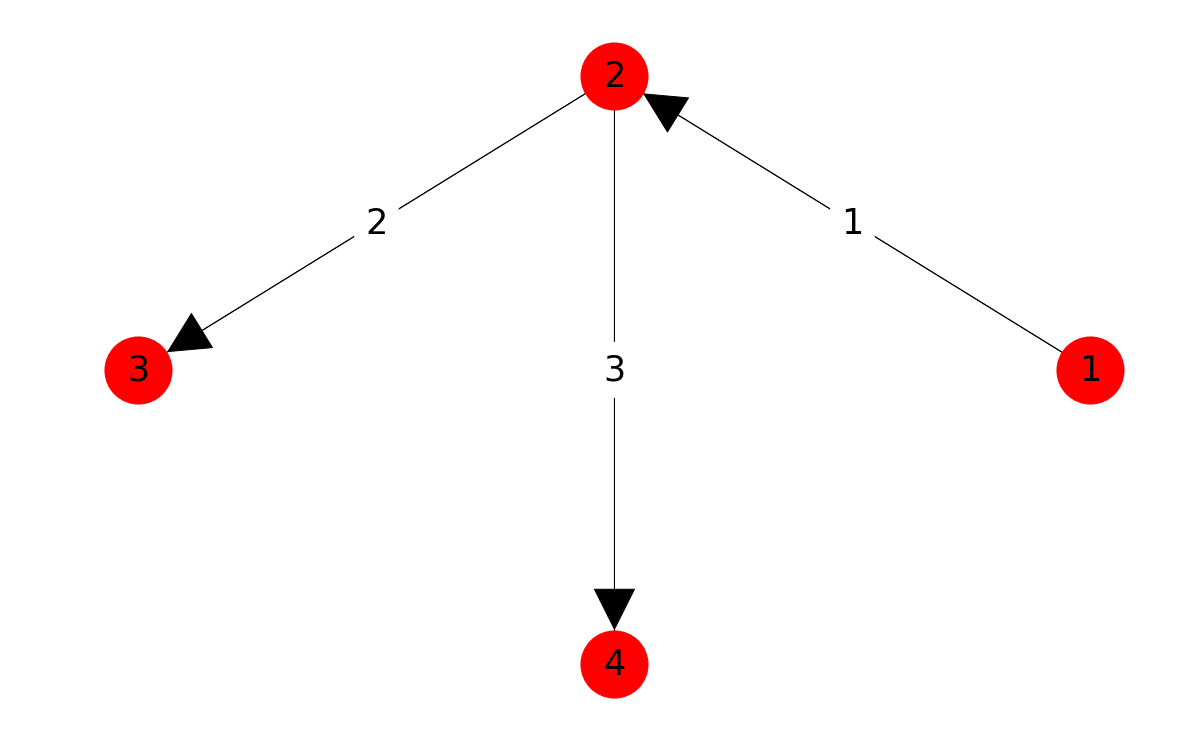
\includegraphics[width=\linewidth]{picts/1.png}
  \caption{Пример графа}
  \label{fig:simple_graphs}
\end{figure}

Ориентация рёбер графа, изображенного на рисунке 2.1, обозначена стрелкой.

Граф $ G $ задаётся множествами $V, E$, соответственно множество вершин (узлов) и множество рёбер.
Таким образом -- $G = (V, E)$
Количество вершин в графе $ G $ -- $ N_V = | V | $ и дуг (рёбер) соотвественно -- $ N_E = | E |.$  

Вершины графа будем обозначать числами натурального ряда $ 1\dots N_V $. Дуги графа принято обозначать латинскими буквами с индексами -- $ a_1 \dots a_{N_E} $.

Говорят, что дуга инцидентна вершине, если она исходит из этой вершины или заходит в неё. Вершины, которым инцидентна только одна дуга, называются висячими.

Полным графом называется граф, у которого любая пара вершин соединена ребром (дугой). В полном графе $ \widetilde G $, число вершин $ N_V = C_{n}^2 = \frac{n (n - 1)}{2} $.

\subsection{Способы представления графов}
Графы, как математический объект, можно задать несколькими способами.
\paragraph{Основные способы}
\begin{enumerate}
\item Матрица (таблица) смежности
\item Список рёбер
\item Матрица инцидентности
\end {enumerate}

Для каждого способа будет приведён пример на основе графа из рисунка 2.1.

\subsubsection{Матрица смежности}
Матрицей смежности для графа $ G = (V, E) $ называется квадратная матрица $ A = (a_{ij}) $, строкам и столбцам которой соответствуют вершины графа. Для неориентированного графа число $ a_{ij} $ равно числу ребер, инцидентных $ i $ и $ j $. Для орграфа (ориентированного, направленного графа) число $ a_{ij} $ равно числу ребер с началом в $ i $ и концом в $ j $.

\[
A = \begin{bmatrix}
    0 & 1 & 0 & 0 \\
    0 & 0 & 1 & 1 \\
    0 & 0 & 0 & 0 \\
    0 & 0 & 0 & 0
\end{bmatrix}
\]

\subsubsection{Список рёбер}
Списком рёбер графа называется таблица, состоящая из двух столбцов, в которой на пересечении $i$-й строки и первого (левого) столбца записывается ребро $ a_i $, а на пересечении $ i $-й строки и второго (правого) столбца записываются вершины, инцидентные ребру $ a_i $.

\[
T = \begin{bmatrix}
    1 & 1, 2 \\
    2 & 2, 3 \\
    3 & 2, 4 \\
\end{bmatrix}
\]

\subsubsection{Матрица инцидентности}
Матрицей инцидентности для графа $ G = (V, E) $ называется матрица $ B = (b_{ij}) $, столбцам которой соответствуют вершины графа, а строкам — ребра. Число ориентированного графа $ b_{ij} $ равно:

\[
	(b_{ij}) = \begin{cases} 
		1, $ если $ a_i $ исходит из $ i \\
		-1, $ если $ a_i $ заходит в $ i \\ 
		0, $ иначе $
	\end{cases}
\]

Для неориентированного:

\[
	(b_{ij}) = \begin{cases} 
		1, $ если $ a_i $ инцидентно $ i \\
		0, $ иначе $
	\end{cases}
\]

Матрица инцидентности для графа из рисунка 2.1 :

\[
B = \begin{bmatrix}
    1 & 0 & 0 \\
    1 & 1 & 1 \\
    0 & 1 & 0 \\
    0 & 0 & 1
\end{bmatrix}
\]

\paragraph{В рамках рассматриваемой работы -- основным способом задания графов будет матрица инцидентности}

\section{Уравнения для анализа и газоснабжения}
Преступим к изучению методов расчета систем газоснабжения. Структуру сети будем изображать в виде направленного графа и использовать соответствующую терминологию.
\paragraph{Расчетом системы} будем называть воспроизведение (моделирование) режимов -- определение расхода по дугам и давления по узлам (вершинам графа). Известными считаются: конфигурация системы и характеристики оборудования.
Перед тем, как приступить к моделированию, необходимо грамотно построить граф системы адекватно отражающий технологическую суть газотранспортной сети. Граф также дополняется данными об оборудовании: диаметры и допустимые давления в трубах, характеристики компрессорных агрегатов, технологические особенности ГРС и т.д.
\paragraph{Расчетная схема} -- информационный комплекс включающий в себя граф системы и формулы для расчета режимов каждого её элемента.
Кроме того, если на расчетной схеме задать индентификационные параметры, то получится \textbf{гидравлическая модель системы}.  

\subsection{Законы течения по трубе}
Для расчета падения давления на участке газовой сети \textbf{среднего и высокого давлений} используется формула
\[ p_s^2 - p_f^2 = \frac{\rho}{81 \pi^2} \lambda  \frac{Q_n^2}{D^5} \rho_n L = 0.12687 10^{-4} \lambda  \frac{Q_n^2}{D^5} \rho_n L  \eqno (1) \]
где $ p_s $ -- абсолютное давление в начале газопровода, МПа; $ p_f $ -- абсолютное давление в конце газопровода, МПа; $ \rho_0 = 1.01325 $; $ \lambda $ -- коэффициент гидравлического трения; $ L $ -- расчетная длина газопровода постоянного диаметра, м; $ D $ -- внутренний диаметр газопровода, см; $ \rho_n $ -- плотность газа при нормальных условиях; $ Q_n $ -- расход газа, при нормальных условиях.
 
Газопроводы \textbf{низкого давления} расчитываются с помощью формулы

\[ p_s - p_f = \frac{ 10^6 }{81 \pi^2} \lambda  \frac{Q_n^2}{D^5} \rho_n L \eqno (2) \]

В отличии от газопроводов среднего и высокого давлений здесь $ p_s, p_f $ измеряется в Па.

\paragraph{Соотношение (1) описывает газовые сети.}

Соотношение (1) можно переписать в так называемой упрощенной форме

\[ P_s - P_f = \Lambda x^2 \]

Здесь через $ P_s, P_f $ обозначены потенциалы потенциалы течения, роль потенциала в (1) играет квадрат давления $ p^2 $; $ \Lambda $ -- обобщенный коэффициент сопротивления. Для сетей газораспределения

\[ \Lambda = c \lambda D^{-5} \rho_0 L \]



\subsection{Первый закон Кирхгофа}
Наряду с расходами по дугам, следует также рассмотреть внешние притоки и отборы $ Q_i $ в узлах системы газоснабжения (СГ) -- вершинах графа. Величину $ Q_i $ будем считать положительной ($ Q_i > 0$).

В случае, когда $ Q_i $ -- приток, то величина берется со знаком '+', если отбор, то со знаком '--'.

Для представления законов Кирхгофа в векторно-матричной форме: вектор узловых давлений $ \overline{\textbf{P}} = || P_j || $, вектор притоков-отборов $ \overline{\textbf{Q}} = || Q_j || $, а также вектор расходов $ \textbf{x} = || x_{j, k} || $ из узла  $ j $, в узел $ k $.

Первый закон Кирхгофа в векторно-матричной форме

\[ \overline{\textbf{A}} \textbf{x} = \overline{\textbf{Q}} \eqno (3) \]

Матрица $ \overline{\textbf{A}} $ - матрица инцидентности графа рассматриваемой системы, \textbf{с исключением последней строки}, так как строки матрицы $ A $ -- линейно-зависимы. 

\subsection{Второй закон Кирхгофа}
Введем $n-$мерный по числу дуг вектор напряжений $ \textbf{y} = ||y_{ik}|| $, положив $ y_{ik} = P_i - P_k $
Второй закон Кирхгофа устанавливает, что алгебраическая сумма напряжений по по любому замкнутому контуру равна нулю. На контуре определяется направление обхода. Алгебраическая сумма -- это значит, что напряжения берутся со знаком '+', если направление контура и дуги совпадают, иначе со знаком '--'.

Если учесть, что $ y_{ik} = \Lambda_{ik} x_{ik} |x_{ik}|$, то получаются соотношения связывающие расходы $ x_{ik} $.

В векторно-матричной форме уравнения второго закона Кирхгофа имеют вид 
\[ \textbf{By} = 0  \eqno (4) \]  

\textbf{B} -- цикломатическая матрица, или матрица контуров.

\section{Постановка расчетной задачи. Граничные условия}

Пусть G -- ориентированный граф с $ N_V $  узлами (образующими множество узлов $ \textbf{V} $) 
и  $ N_E $ ветвями (образующими множество ветвей $ \textbf{E} $). Расход по $ i $-й ветви связан 
с начальным и конечным давлениями  $ p_s^i $ и $ p_f^i $ замыкающим соотношением

\[ x_i = \phi \left ( p_s^i, p_f^i \right) \eqno (5) \]
$ \textbf{Q} $ - вектор узловых 
притоков. Тогда уравнения Кирхгофа (уравнения балансов в узлах) записывается в виде

$ \textbf{A} $ - матрица инцидентности графа $ G $
$ (a_{ij} = 1 $, если ребро j начинается в узле i, $ a_{ij} = -1 $, если ребро j заканчивается в узле i);

$$ \textbf{AX} = \textbf{Q} \eqno(6) $$

Используя матрицы $ A_S $ и $ A_F $, соответствующие выходящим и входящим ветвям ($ A = A_S + A_F $), 
вектор узловых давлений  $ P $ и вектор $ \Phi $ функций $ \phi_i $, уравнения (1) можно
записать в виде

$$ P_S = A_S^T P, P_F=-A_F^T P $$
$$ X = \Phi(P_S, P_F) \eqno(7) $$

Преположим что граничные условия заданы 

$$ P_{\gamma} = ( P_{i_1}, \dots, P_{i_k} ), Q_{\gamma} = ( Q_{i_{k + 1}}, \dots, Q_{i_{n}} ) \eqno(8) $$

Таким образом система уравнений

$$ X = \Phi (P_S, P_F), \\ \widetilde A X = Q \eqno (9)$$

Матрица $ \widetilde A $ - это матрица $ A $, только без последней строки, так как $ rank A = min(N_E, N_V) = N_V - 1 $.

При граничных условиях (8), система (9) имеет единственное решение. 

После решения системы (9), получаются векторы $ Q_0 $, $ P_0 $

Затем, предположим, что граничные условия (8) -- получили малые приращения соответственно 
$$ \widetilde P_{\gamma} = P_{\gamma} + \delta P_{\gamma},  \widetilde Q_{\gamma} = Q_{\gamma} + \delta Q_{\gamma} $$
Требуется оценить влияние изменений граничных условий на неграничные (незаданные) переменные.

\section{Матрица чувствительности}
Для удобного рассмотрения модели введем обозначения:

$ V_P $ -- множество узлов с заданным давлением,
$ V_Q $ -- множество узлов с заданным притоком

Рассмотрим случай, когда замыкающие соотношения являются непрерывно диффиренцируемыми в окрестности
решения $ P_0, Q_0 $ системы (5).

Обозначим 

$$ d_{Si} = \frac{\partial \phi_i(P_S, P_F) }{\partial P_S} $$

$$ d_{Fi} = -\frac{\partial \phi_i(P_S, P_F) }{\partial P_F} $$

Тогда в силу монотонности $ \phi_i $ справедливы неравенства $ d_{Si} \geq 0 $ и $ d_{Fi} \geq 0 $

Определим диагональные матрицы $ D_S $ и $ D_F $ с $ d_{Si} $ и $ d_{Fi} $ на диагонали.
Тогда уравнения (2) и (3) можно переписать 

$$ dX = (D_S A_S^T + D_F A_F^T) dP \eqno(7) $$
$$ dQ = A (D_S A_S^T + D_F A_F^T) dP \eqno(8) $$

Перенумеруем узлы графа так, чтобы сначала шли узлы с заданными притоками (из $ V_Q $), 
а затем с заданными давлением (из $ V_P $) и разобьем векторы и матрицы на соответствующие
блоки:

$$ P = \left(\frac{P_{var}}{P_{fix}}\right) Q = \left(\frac{Q_{var}}{Q_{fix}}\right) A = \left( \frac{A_Q}{A_P} \right) A_S = \left( \frac{A_{SQ}}{A_{SP}} \right) A_F = \left( \frac{A_{FQ}}{A_{FP}} \right) \eqno(9) $$

Тогда уравнения (7) и (8) можно переписать 

$$ dX = (D_S A_{SQ}^T + D_F A_{FQ}^T)dP_{var} + (D_S A_{SP}^T + D_F A_{FP}^T)dP_{fix} \eqno(10) $$
$$ dQ_{fix} = A_Q (D_S A_{SQ}^T + D_F A_{FQ}^T)dP_{var} + A_Q ( D_S A_{SP}^T + D_F A_{FP}^T)dP_{fix} \eqno(11) $$
$$ dQ_{var} = A_P (D_S A_{SQ}^T + D_F A_{FQ}^T)dP_{var} + A_P ( D_S A_{SP}^T + D_F A_{FP}^T)dP_{fix} \eqno(12) $$

Матрица $ M = A_Q (D_S A_{SQ}^T + D_F A_{FQ}^T) $ связывает подвекторы с фиксированными переменными (заданными граничными условиями) с подвекторами свободных переменных.
Эта матрица также называется модифицированной матрицей Максвелла или $M$-матрицей.

Отметим еще несколько матриц
$$ M_{PP} = A_P ( D_S A_{SP}^T + D_F A_{FP}^T) \eqno(13) $$ 
$$ M_{PQ} = A_P ( D_S A_{SQ}^T + D_F A_{FQ}^T) \eqno(14) $$
$$ M_{QP} = A_Q ( D_S A_{SP}^T + D_F A_{FP}^T) \eqno(15) $$

Тогда (11) и (12) можно переписать используя (13), (14) и (15)
$$ dQ_{var} = M_{PQ} M^{-1} dQ_{fix} + ( M_{PP} - M_{PQ} M^{-1} M_{QP} )dP_{fix} \eqno(16) $$
$$ dP_{var} = M^{-1} dQ_{fix} - M^{-1} M_{QP} dP_{fix} \eqno(17) $$

Заметим также, что матрицы $$ M, M_{QP}, M_{PQ}, M_{PP} $$ -- функциональные матрицы, векторных аргументов $ P_0, Q_0 $